\documentclass[a4paper,11pt]{article}
\usepackage{graphicx}
\usepackage[T1]{fontenc}
\usepackage[utf8]{inputenc}
\usepackage{lmodern}
\usepackage{float}
\usepackage[lofdepth,lotdepth]{subfig}
\usepackage[english]{babel}
\usepackage[margin=1in]{geometry}
\usepackage{wrapfig}

\title{Statistical Mechanics Project}
\author{Adam Lamson\\
Department of Physics\\
University of Colorado Boulder\\
\texttt{Adam.Lamson@colorado.edu}}
\date{4/29/16}

\begin{document}

\maketitle

\begin{center}
\end{center}

\tableofcontents

\begin{abstract}
    In this project we simulate a 2-D finite Ising model with periodic boundary conditions and a square unit cell. The Ising Model Hamilitonian is given by
    \begin{equation}
        \mathcal{H} = -J \sum_{\langle ij \rangle} s_i s_j - H\sum_i s_i
    \end{equation}
    where $s_i$ represents the spin of particle i with a value of $\pm1$, $J$ is the strength of the coupling between adjacent particles, and $H$ is the strength of external magnetic field. In the canonical enssemble a system of V\footnote{$V=L*L$ where L is the number of particle per side of a unit cell.} particles can be defined by the values of $J$, $H$, and kT\footnote{The temperature of the ensemble multiplied by the boltzmann factor. We will simply refer to this as T for the rest of the paper.}. From these we can determine quantities such as the energy, magnetization, and susceptibility of each system. The energy, $E$, simply uses the above Hamilitonian while the magnetization is simply defined as 
    \begin{equation}
        M = \sum_i s_i
    \end{equation}
The susceptibility of the system is then defined as 
    \begin{equation}
        \chi = \frac{\partial M}{\partial H}\bigg\vert_T 
    \end{equation}

    In 2-D there is an analytical solution for the Ising Model, however, this proves overly complicated most of the time. An easier approach in the modern day is to use very simulation techniques to obtain the above calculated values. I created a python program(attached) that implemented both the heat bath and metropolis algorithm to thermalize a system of volume V. To find the critical temperature, $T_c$, a logarithmic slice of temperatures was taken from .01 to 100 with $J=1$ and $H=0$. Once the two values that showed the transition from highly ordered to disordered was identified a linear slice was taken to find critical temperature to higher and higher degrees of accuracy. This showed strong correlation to the known value of $T_c \approx 2.269$. Anti-ferromagnetic behavior was seen for negative values of $J$ but most measurements were conducted with $J=1$.

\end{abstract}

\section{The 2-dimensional Ising model}

    \subsection{Thermalization of $E$ and $M$}

        \paragraph{Initial Tests}We begin by showing that at low temperatures systems will have spins that are all strongly correlated while at higher temperatures this correlation fades.

        \begin{figure}[H]
            \centering
            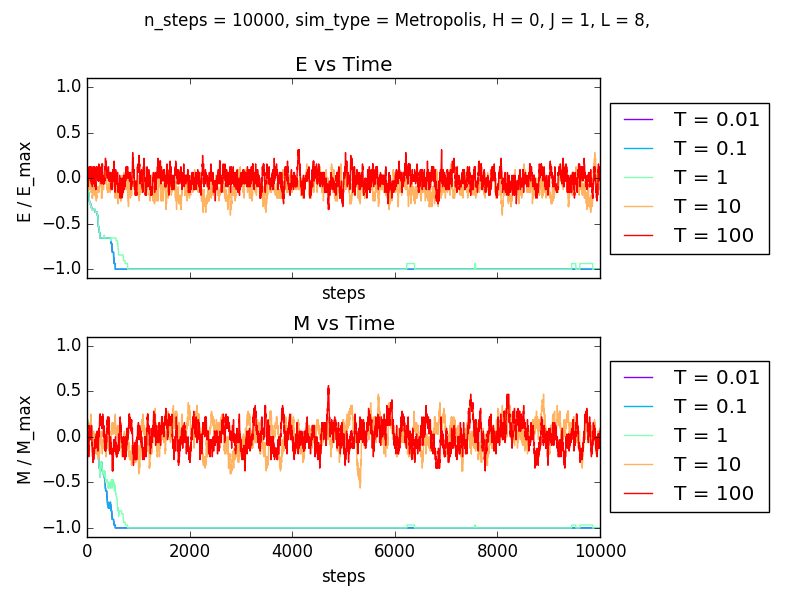
\includegraphics[width=.75\textwidth]{Graphs/Large_Temp_slice.png}
            \caption{Time evolution of system of 64 particles showing the different behaviours at various temperatures. E = Energy and M = Magnetization} 
        \end{figure}

        As expected we see two regimes emerge with $T \le 1$ showing a steady state of lowest energy and relatively constant magnetization while $T \ge 10$ random distributions around 0 for both magnetization and energy. From this we can deduce that the critcal Temperature, $T_c$, where systems will go from having spins correlated to being uncorrelated in orientations, exists between 1 and 10. 


        \paragraph{Finding $T_c$} We can look at the average energy and magnetization of runs at various temperatures to find the transition and thus the critical temperature.
        
        \begin{figure}[H]
            \centering
            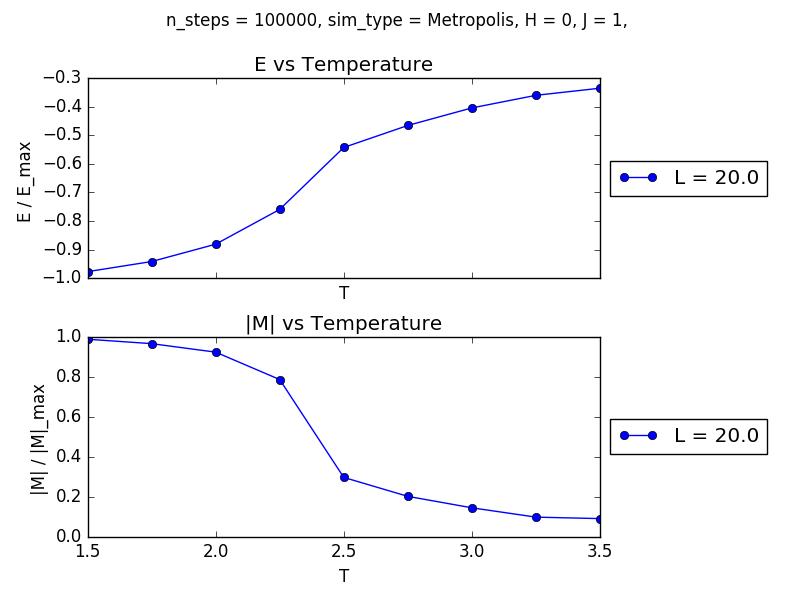
\includegraphics[width=.75\textwidth]{Graphs/Find_Tc_slice_2_good.png}
            \caption{}
        \end{figure}



    \subsection{Depedence on $H$}

    \subsection{Tunneling}

    \subsection{Difference of Algorithms}


\section{Ising Fluctuations and Susceptibilities}

    \subsection{Correlations and Susceptibilities: Analytical}

    \subsection{Correlations and Susceptibilities: Numerical}

    \subsection{Low Temperature Expansion for the Magnetization}

    \subsection{High Temperature Expansion for the Magnetization}


\section{Last part of the project}

    \subsection{Specific Heat: Analytical}

    \subsection{Specific Heat: Numerical}

    \subsection{Finite Size Scaling}

\end{document}

